\documentclass[times, utf8, seminar, numeric]{fer}
\usepackage{booktabs}
 \usepackage{url}

\begin{document}

% Ukljuci literaturu u seminar
\nocite{*}

% TODO: Navedite naslov rada.
\title{Faza konsenzusa u OLC paradigmi sastavljanja genoma – Sparc}

% TODO: Navedite vaše ime i prezime.
\author{Nikola Bukovac, Vinko Kolobara}

% TODO: Navedite ime i prezime voditelja.
\voditelj{Mile Šikić}

\maketitle

\tableofcontents

\chapter{Uvod}
DNK je važna sastavnica svakog živog bića s obzirom da sadrži svu biološku informaciju svake jedinke, što je jedan od razloga zašto ju znanstvenici pokušavaju što preciznije očitati. Današnji uređaji su dovoljno brzi i jeftini, ali problem predstavljaju kratka očitanja koja je moguće napraviti s takvim uređajima, te se stoga razvijaju i algoritmi koji će dobivena očitanja pokušati spojiti u jedan slijed.

Danas je jedna od najraširenijih metoda sekvenciranja genoma takozvana \emph{shotgun} metoda sekvenciranja kod koje se DNK cjepka slučajnim načinom na male dijelove na različitim pozicijama i različitim duljinama što dovodi do nepreciznosti samih očitanja DNK pa je taj proces potrebno provoditi nekoliko puta nad istim dijelovima za kvalitetnu rekonstrukciju DNK. Uređaji koji se danas pretežno koriste pripadaju drugoj generaciji uređaja za sekvenciranje, koji iakosu jako precizni ostvaruju jako male dužine očitanja, veličine do nekoliko stotina parova nukleotida što značajno usporava sami proces očitavanja. Kako bi se doskočilo ovom problemu razvijena je treća generacija uređaja koja može očitati 5 do 120 tisuća parova nukleotida u jednom čitanju, ali veliki problem predstavlja jako velika pogreška u očitanju koja iznosi od 15\% do 50\%.

Probleme koji nastaju pri očitavanju genoma rješavamo s algoritmima sastavljanja genoma te tako spajamo kraća očitanja i popravljamo nastale greške kod očitanja. Moderni algoritmi koji se bave ovim problemom temelje se na grafovim, a najkorištenije su dvije metode: \emph{Preklapanje-Razmještaj-Konsenzus} metoda temeljena na grafu preklapanja ili metoda temeljena na \emph{k-mer/de Bruijn} grafovima \cite{sikic2013bioinformatika}.

Cilj ovog rada je upoznavanje, implementacija te analiza implementiranog algoritma faze konsenzusa u OLC paradigmi sastavljanja genoma, naziva Sparc. Postavljeni ciljevi nam određuju i samu strukturu rada pa je tako u drugom poglavlju , opisana ideja algoritma Sparc te prikazan grafički primjer koji prikazuje način na koji algoritam radi. Treće poglavlje opisuje kako smo ostvarili našu implementaciju algoritma te što smo sve koristili za nju. Četvrto poglavlje donosi našu analizu rješenja koje smo implementirali te način na koji smo ju proveli.

%=========================================================================
%Početak drugog poglavlja
%=========================================================================

\chapter{Sparc algoritam}
Algoritam Sparc je algoritam faze konsenzusa u Preklapanje-Razmještanje-Konzenzus (engl. \emph{Overlap-Layout-Consensus, OLC}) paradigmi sastavljanja očitanja genoma. Kao temelj algoritma se koristi de Bruijn/k-mer graf nad kojim se potom provodi ostatak algoritma \cite{Ye2016}.
\section{Opis algoritma}
Prvi korak algoritma je konstrukcija k-mer grafa na temelju predanog ulaza koji sadrži izlaz iz faze Razmještaja, OLC metode. Ovisno o parametrima \emph{k} i \emph{g} kreira se inicijalni k-mer graf, gdje navedeni parametri određuju strukturu grafa, konkretno \emph{k} specificira koliko će nukleotida biti sadržano u pojedinom čvoru grafa, a \emph{g} specificira koliko će se nukleotida nalaziti na svakom bridu. Inicijalni graf je usmjeren sa samo jednim bridom iz svakog vrha osim zavšnog, koji ga nema. Razlika između ovog grafa i klasičnog de Bruijn grafa je u to tome što su isti k-meri na različitim pozicijama nezavisni jedni od drugih dok su kod de Bruijn grafa smješteni u jednom vrhu pa se ovaj graf smatra \emph {sparse} grafom. Sljedeći korak algoritma je poravnjanje dodatnih slijedova čiji se postupak se provodi ovisno o tome da li k-mer u novom slijedu odgovara k-meru u originalnom slijedu i njegovom bridu gdje se onda samo poveća težina brida za definiranu težinu ili ukoliko ne odgovara dodaje se novi brid u graf i kreira se dodatni k-mer i samim time kreira se novi put u grafu. Ovaj postupak je jako sličan kreiranju de Bruijn grafa, ali zbog razlikovanja istih k-mera ovisno p njihovoj poziciji, postoji razlika u postupku. Ovaj korak se ponavlja za sve slijedove koje smo dobili sekvenciranjem. Završni korak Sparc algoritma je traženje puta u grafu koji ima najveću težinu, što je zahvaljujući činjenici da je konstruirani graf usmjeren i acikličan moguće napraviti s BFS ili DFS algoritmom kojim računamo težinu svakog vrha u grafu. Rekonstrukcija slijeda se provodi tako da krenemo od najtežeg vrha i vraćamo se po najvećim težinama natrag sve do početnog vrha. Kompleksnost algoritma...

\section{Primjer}
\begin{figure}[htb]
	\centering
	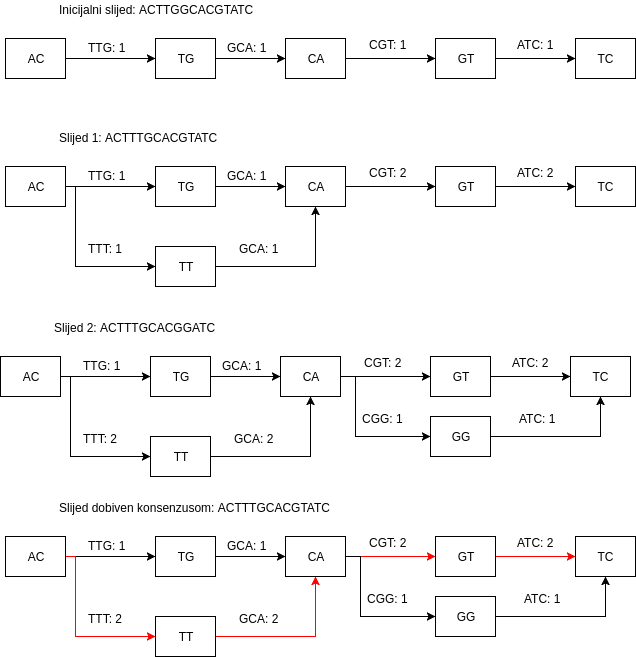
\includegraphics[scale=0.6]{images/backbone.png}
	\caption{Postupak izgradnje grafa s k=2, g=3}
	\label{picture:example}
\end{figure}

Slika \ref{picture:example} prikazuje cjelokupni postupak algoritma Sparc. Inicijalni slijed služi za kreiranje inicijalnog lanca (engl. \emph{backbone}). Nakon kreiranja \emph{backbone}-a grafa, sljedeći slijed poravnavamo tako da krećemo od početka slijeda i vidimo da je prvi k-mer AC jednak k-meru kontruiranom u grafu, ali je prijelaz na sljedeći k-mer TTT različith od onoga koji se već nalazi u grafu te je stoga potrebno konstruirati novi k-mer TT te novi brid iz k-mera AC prema novom k-meru TT, a taj brid je TTT. Slijedećih g nukleotida je GCA koji trebaju završiti u k-meru CA koji već postoji u konstruiranom grafu te je potrbno kreirati brid CGA od k-mera TT prema k-meru CA. Sljedećih g nukleotida je CGT, budući da taj brid postoji u konstruiranom grafu potrebno je samo povećati težinu postojećeh brida, isto vrijedi i za sljedećih g nukleotida ATC. Postupak je jednak i za slijed 2. Za određivanje najtežeg puta pratimo bridove s najvećim težinama, a u ovdje kontruiranom grafu to je put od k-mera AC bridom TTT potom bridom GCA, CGT i ATC te je stoga rekonstruirani slijed ACTTTGCACGTATC.

%=======================================================================
%Početak trećeg poglavlja
%=======================================================================

\chapter{Naša implementacija algoritma}
Za ostvarivanje naše implementacije algoritma faze konzensuza Sparc, koristili smo programski jezik C++ uz korištenje dodatnih biblioteka i alata, koji će biti navedeni u nastavku. Implementacija koristi specifične formate podataka koji su također opisani u nastavku.
\section{Korišteni formati podataka}
Sve podatke o slijedovima koje koristimo u našem algoritmu se nalaze u predodređenim formatima podataka kako bi se algoritam mogao što jednostavnije koristiti u opće svrhe. Korišteni formati podataka i način njihova korištenja opisan je u nastavku.
\subsection{FASTA}
Naš algoritam ovaj format koristi kako bi napravio početni slijed (engl. \emph{backbone}) za ulaz te na izlaz stavlja rekonstruirani slijed također u FASTA formatu.
Ulaz u naš algoritam je u biti izlaz iz faze razmještaja OLC metode.
\subsection{FASTQ}
Sličan FASTA formatu, ali osim samog slijeda sadrži i oznaku kvalitete svakog očitanja.
Ovaj format podataka sadrži sekvencirane slijedove koji će poslužiti za rekonstrukciju originalnog slijeda.
Iako naša implementacija ne koristi direktno ovaj format podataka, on se koristi kao ulaz za alat graphmap koji služi za generiranje SAM formata podataka.
\subsection{SAM}
Ovaj format podataka sadrži grupirane informacije o svim očitanjima iz FASTQ formata podataka. Podaci iz ovog formata podataka služe za rekonstrukciju genoma. 

Podaci iz SAM formata podataka koje koristimo u našoj implementaciji su:
\renewcommand{\labelitemi}{$\bullet$}
\begin{itemize}
	\item FLAG - skup zastavica koje ovisno o vrijednosti utječu na naš algoritam. Vrijednost zastavice 4 označava da je trenutno mapiranje loše te ga stoga preskačemo, također uzimamo i vrijednost zastavice 16 koja označava da je trenutno slijed U SEQ dijelu u inverznom poretku te ga onda komplementiramo. Ostale vrijednosti zastavica zanemarujemo.  
	\item POS - pozicija na osnovnom slijedu na kojoj počinje trenutno mapiranje, pozicija je indeksirana od indeksa 1
	\item CIGAR - popis operacija koje su napravljene nad očitanjem kako bi se dobilo mapiranje
	\item SEQ - originalno očitan slijed, prije nego što su obavljene CIGAR operacije
\end{itemize}

\section{Korištene biblioteke}
Osim standardnih biblioteka programskog jezika C++, kao što su na primjer biblioteke za I/O operacije te STL(\emph{Standard Template Library}) biblioteke koja sadrži implementacije složenijih struktura podataka, koristili smo i biblioteku/alat GraphMap.
\subsection{GraphMap}
GraphMap biblioteka pruža implementaciju mapiranja poravnanja očitanih slijedova u odnosu na početni slijed. Ovu biblioteku smo koristili kako bi dobili poravnjanja slijedova koja onda koristimo kod Sparc algoritma za konstruiranje grafa. Mapiranja poravnjanja se dobiju tako što se GraphMap alatu predaju slijed na kojem želimo raditi poravnanje u FASTA formatu te datoteku s očitanjima slijedova u FASTQ formatu. Korištenjem opcije \emph{align} dobiju se mapiranja poravnanja u SAM formatu datoteke.
GraphMap alat nismo koristili direktno u našoj implementaciji, ali smo koristili nastala mapiranja kako bi napravili što efikasniji algoritam.

\section{Struktura implementacije}
Implementacija je rasčlanjena na nekoliko cjelina: glavni program, definicije formata i njihove parsere te dio u kojemu je definirana struktura k-mer grafa kao i implementacija samog Sparc algoritma.

Datoteka \emph{main.cpp} predstavlja glavni program u kojemu se instanciraju potrebne klase za provedbu algoritma kao i svi potrebni parseri koje koristimo 

\section{Instalacija i pokretanje algoritma}
Objašnjenje kako se implementacija instalira i pokreće

%===========================================================================
% Početak četvrtog poglavlja
%==========================================================================

\chapter{Analiza implementacije}
Za utvrđivanje kvalitete implementacije, radimo usporedbu slijeda koji smo koristili kao ulaz u algoritam te slijeda koji smo dobili kao izlaz iz algoritma što radimo tako što oba slijeda uspoređujemo s referentnim slijedom koji nam služi za određivanje koliki je postotak podudarnosti ulaznog i izlaznog slijeda s referentnim. Postotak podudarnosti slijedova nam je najbitniji podatak prilikom analize, ali jednako tako su nam važni i podaci o utrošku memorijskog prostora te vremenu izvođenja algoritma.


\section{Alati za analizu}
Kako bi analiza podataka bila što preciznija koristimo gotove alate, kojima provjeravamo prije navedene čimbenike koje pratimo.

\subsection{DnaDiff}
DnaDiff je jedan od alata iz programskog paketa otvorenog koda MUMmer, koji osim alata DnaDiff sadrži i druge alate koji se koriste na području bioinformatike. DnaDiff radi analizu između dva genetska slijeda i utvrđuje njihovu sličnost. Analiza provedena alatom daje detaljne informacije o sličnostima slijedova, ali kao faktor kvalitete implementacije smo koristili podatke iz datoteke \emph{out.report} i poglavlja o sličnosti poravnanja, \emph{Alignments}. Navedeno poglavlje ima analizu za 1-1 i M-M poravnanja koja su prilikom naših testiranja u većini slučajeva za polje AvgIdentity bila identične ili gotovo identične vrijednosti pa smo stoga kao faktor kvalitete rješenja odlučili koristiti vrtijednost pod 1-1 AvgIdentity.

\subsection{cgmemtime}
Alat cgmemtime služi za analizu vremena i potrošene memorije. Za memoriju se ispisuje najveća zabilježena vrijednost za vrijeme izvođenja algoritma te tako imamo informaciju koliko je minimalno memorije potrebno rezervirati za izvođenje programa.


\section{Testna konfiguracija}
Osnovni podaci o računalnoj konfiguraciji koja je korištena za analizu izvođenja ostvarenog rješenja navedena je u nastavku:
\renewcommand{\labelitemi}{$\bullet$}
\begin{itemize}
	\item Operacijski sustav - Arch Linux x86 64
	\item Procesor - Intel Core i3-6100 @ 3.70GHz
	\item RAM - 16 GiB DDR4 @ 2133MHz
\end{itemize}

\section{Analiza kvalitete rješenja}
\begin{table}[htb]
	\centering
	\begin{tabular}{l|ll}
		& \multicolumn{1}{l}{lambda} & ecoli \\ 	\hline
		layout 				& 86.16 	& 88.57 \\ 	\hline
		naš 1. iteracija  	& 91.00     & 95.71 \\	\hline
		naš 2. iteracija  	& 91.13     & 95.80 \\	\hline
		original 1.iteracija   &    -         & -\\ \hline
		original 2.iteracija   &    -         & -
	\end{tabular}
	\caption{Usporedba naše implementacije sa slijedom iz faze razmještanja (layout) i referentnim radom (Sparc) nakon prve i druge iteracije algoritma za k=3 i g= 4.}
	\label{table:kvaliteta}
\end{table}

Tablica \ref{table:kvaliteta} prikazuje usporedbu naše implementacije i implementacije referentnog rada iz koje je vidljivo...

\section{Analiza utroška memorije i vremena}
\begin{table}[htb]
	\centering
	\begin{tabular}{l|ll}
		& \multicolumn{1}{l}{vrijeme[s]} & memorija[MiB] \\ 	\hline
		lambda			& 0.28		& 60 	\\ 	\hline
		ecoli  			& 63.70     & 8000  \\	\hline
	\end{tabular}
	\caption{Analiza utroška vremena i memorije za provedbu algoritma za k=3 i g= 4.}
	\label{table:memorija}
\end{table}

Tablica \ref{table:memorija} prikazuje potrošnju memorije i vrijeme izvođenja naše implementacije algoritma i iz nje je moguće vidjeti da su zadovoljena zadana ograničenja za oba skupa podataka. 

%=====================================================================
% Ostatak poglavlja
%=====================================================================

\chapter{Zaključak}
Zaključak.

\bibliography{literatura}
\bibliographystyle{fer}

\chapter{Sažetak}
Sažetak.

\end{document}
